\section{Motivation and Problem Statement}
With the development of wireless access technology as well as the explosion of mobile devices (such as smartphones and tablets), the next generation mobile network is not only restricted to provide the traditional voice services but also the data services. In other words, it is evolving towards all-IP systems. In fact, the mobile data services have become an essential part of many consumers' lives \cite{cisco_forecast,data_services}. So far, users are using their mobile devices not only for personal life but also for work on a regular basis \cite{cisco_service,morgan_stanley, mobile_2010}. As a result, the mobile data traffic has been almost doubled each year during the last few years\footnote{The increasing traffic is mainly driven by mobile video traffic} \cite{cisco_forecast, ericsson}. This trend is expected to continue in the upcoming years, especially with the deployment of fourth generation (4G) networks. Despite the increasing volume of traffic, the average revenue per user is falling fast \cite{mobile_europe}. In addition, in all-IP mobile networks as mobile nodes may frequently change their point of attachment to the IP network, IP mobility management is a crucial concept to meet the demand of ubiquitous Internet connectivity as well as new service requirements such as seamless handover across heterogeneous networks, consistent quality of experience and stringent delay constraints. Mobility can be handled at different layers of protocol stack ranging from the link layer to the application layer, however, most of these mobility management protocols are located at the network layer. Mobile IPv6 (MIPv6), the first mobility protocol standardized by the Internet Engineering Task Force (IETF) for IPv6 networks, maintains the mobile node (MN)'s reachability when it is away from home. It is done by relying on a central mobility, namely Home Agent (HA). However, in MIPv6, the MN needs to perform the mobility-related signaling, that means the MIPv6 protocol stack is required at the MN. It is the main obstacle of the deployment of MIPv6 in the real world. For this reason, Proxy Mobile IPv6 (PMIPv6), as a network-based mobility management, helps to avoid the additional deployment in the MN so that the MN can be kept simple. In other words, mobility can be transparently provided to all legacy MNs. \\

The mobile network operators are being challenged by the increase of mobile data traffic (especially the video traffic) and the new requirements e.g., providing connectivity anywhere and at anytime with consistency of user experience, while preserving the economics of their networks and creating new opportunities for revenue growth. Faced with these challenges, the operators are seeking for innovative solutions to improve their network performance and efficiency, as well as to reduce the costs expended on network operation and maintenance. Two major focuses are: i) increasing the capacity of wireless communication systems;  and ii) designing and implementing an efficient system to deliver the data. Regarding the first aspect, further dramatic increases in radio capacity of mobile broadband will come with the implementation of new wireless technologies such as Worldwide Interoperability for Microwave Access (WiMAX), High Speed Packet Access (HSPA) and Long Term Evolution (LTE). However, spectrum for operators is both limited and expensive. Thus, they are looking at different methods to increase the system capacity such as deploying femto and pico cells, together with selecting the offload traffic between the licensed and unlicensed spectrum (e.g., from 3G to WiFi). Considering the second aspect, the aim is to simplify the network architecture as well as optimize the data transmission costs. Accordingly, the mobile network is currently evolving towards flat architecture. One example is Local IP Access/Selected IP Traffic Offload (LIPA/SIPTO) architecture defined by the 3rd Generation Partnership Project (3GPP). Following the same idea, IETF has recently chartered the Distributed Mobility Management (DMM) working group which specifies the solutions to address the problems and limitations of the current centralized mobility management. In fact, the conventional IP mobility management (e.g., MIPv6 and PMIPv6) leverages on the centralized mobility management approach, thus,  raises several issues for the network operators like inefficient use of network resources, poor performance, and scalability issues when considering a large number of mobile devices and their traffic demand \cite{DMM_requirements, DMM_issues,DMM_problem_statement}. DMM is one of the solutions to help the mobile operators address these limitations while enhancing the overall customer experience.  \\


As Internet is widely deployed and spread across a large area, it carries a variety of common information resources and services. In a sharing world, the group communication service, which refers to the ability to send data to several receivers at the same time, is naturally becoming more and more important especially in some areas like multimedia distribution, gaming, and financial services, etc. In this context, the scalability and bandwidth efficiency from the multicast routing make the IP multicast a remarkable solution from the application point of view to allow the mobile networks to deal with a huge number of traffic, particularly, in mobile environments where users usually share frequency bands and limited capacity \cite{Multicast_MIPv6}. But one of the major challenges for multicast support is when mobility is considered. It comes from the fact that the multicast protocols were designed to support the stationary multicast parties. As such, it raises some issues as a result of the interaction of IP multicast and IP mobility protocols e.g., transparency, routing optimization, packet duplication, service disruption, packet loss and group leave latency, etc \cite{Multicast_MIPv6, multicast_challenges_solutions}.\\
 
Regarding the IP mobile multicast, after more than a decade of research and development efforts, many approaches have been proposed, but most of them are based on such host-based mobility management protocols as MIPv6, Fast Mobile IPv6 (FMIPv6) and Hierarchical Mobile IPv6 (HMIPv6). However, the main drawback of these protocols is that they require the MN to modify its IP stack to participate into the mobility signaling process. In fact, it is the major obstacle of the deployment of MIPv6 in the real world. Additionally, the previous IP multicast approaches cannot be directly applied in a network-based mobility management in which the MN is unaware of mobility process. To solve the aforementioned issues, the IETF has worked in different solutions highlighting the difference between the source and the listener multicast mobility problems in PMIPv6. However the proposed solutions remain unable to address the issues of scalability, performance optimization and compatibility with unicast mobility at the same time. In DMM, there is no complete solution for the multicast mobility support.\\

It is generally acknowledged that a proposed solution cannot be widely accepted without results from valid experimentation. Such validation nowadays can be obtained through various methods, each with its own advantages and limitations. Within the networking field of research, the results’ reliability is one of the most critical issues. Thus, the results credibility is directly related to the methods used, therefore improving them becomes of great importance. In this context, the most widely used method - simulation - sometimes lacks credibility. The lesser used but most credible method - real testbed - is too expensive and difficult to scale and manage. \\

In this thesis, our objective is to deal with the multicast-related issues raised when a multicast node moves in a network-based mobility management domain. In other words, the aim of this research is to find solutions that ensure:
\begin{itemize}
\item Keeping the MN unaware of mobility from the multicast service point of view;
\item Minimizing the service disruption time to even satisfy the strict requirements for the interruption- and delay-sensitive services;
\item Keeping the signaling/tunneling overhead as low as possible;
\item Maximizing the available network resource (reducing the waste of resources and packet duplication), keeping the reliability and improving the scalability of the system;
\item Minimizing the modifications of the mobility management and the multicast routing protocols to support IP mobile multicast. 
\end{itemize}
\begin{figure}[h!] 
 \begin{center} 
 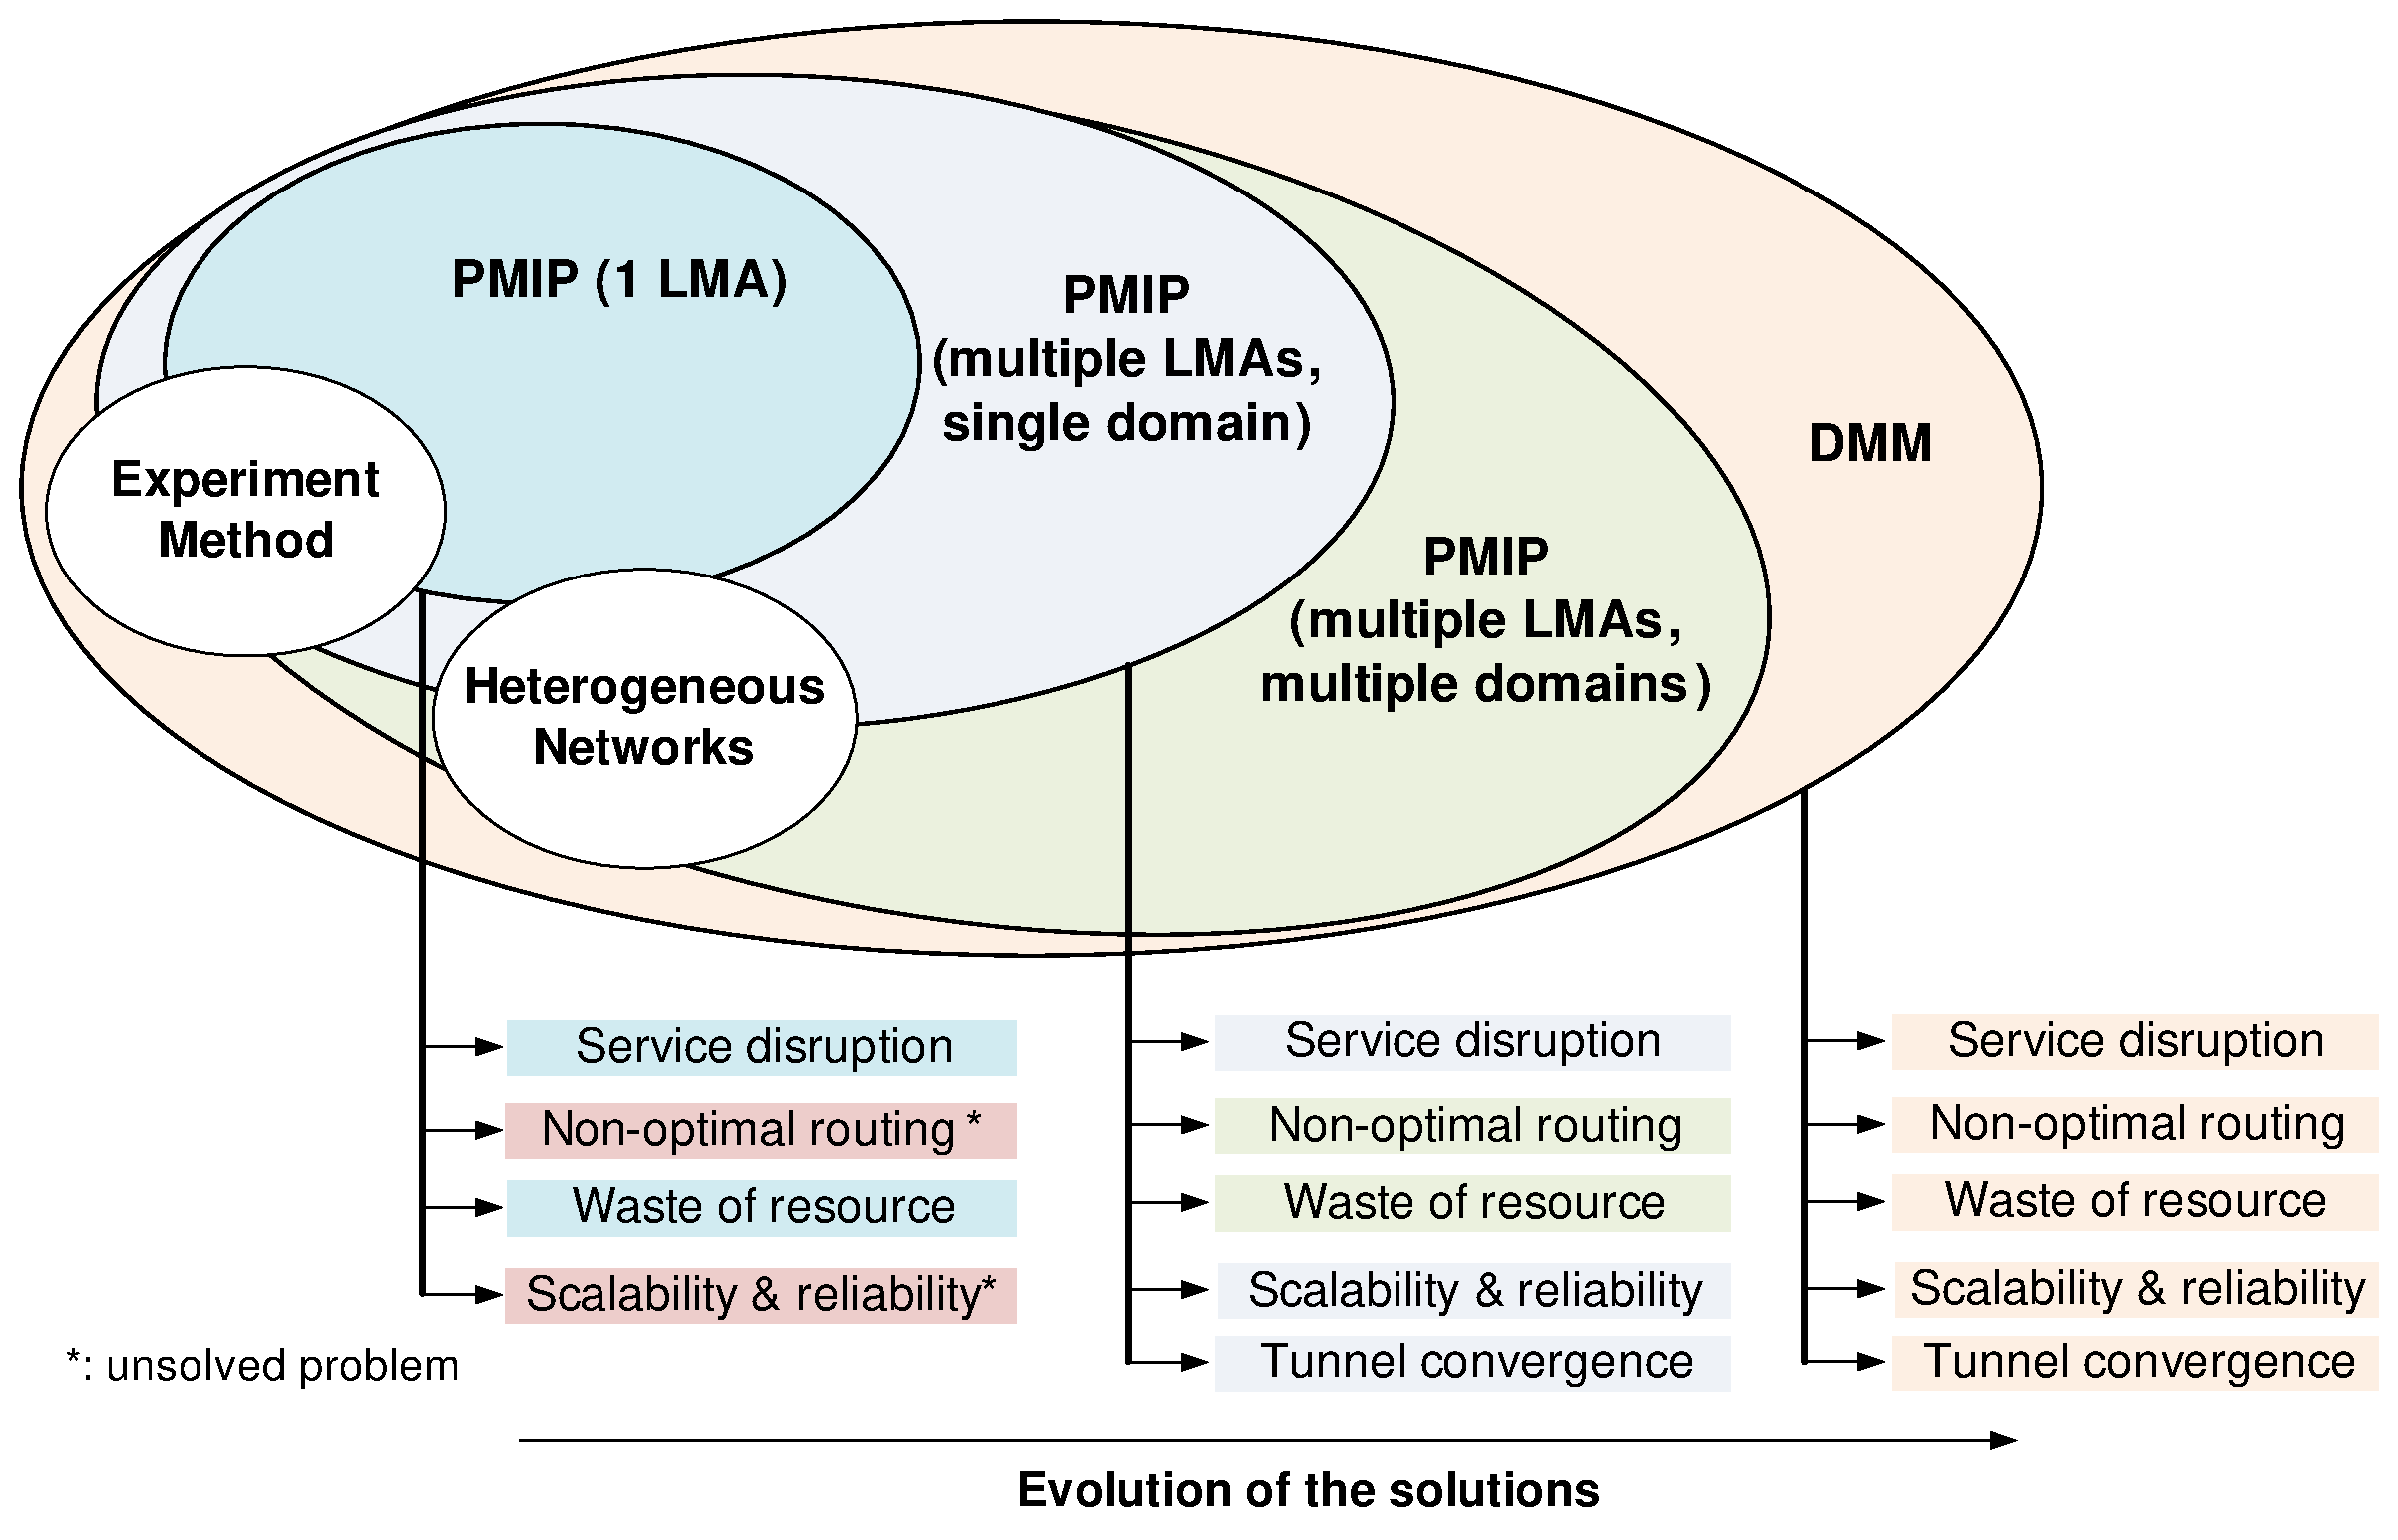
\includegraphics[width=0.72\textwidth]{./Introduction/Chapter1/figures/vision.eps} 
    \caption{Evolution of the solutions for multicast mobility.}
     \label{fig:vision}
  \end{center} 
\end{figure}
The evolution of the solutions for multicast mobility is illustrated in Fig.~\ref{fig:vision}. For a single PMIPv6 domain (with one local mobility anchor (LMA)), we introduce a method to minimize the service disruption time considering both cases: a mobile node with single or multiple interfaces. The waste of resources caused by a long leave latency is also reduced. On the other hand, the non-optimal routing; scalability and reliability issues are unsolved. Considering a single PMIPv6 domain with multiple LMAs, an additional issue is introduced - the tunnel convergence problem (or packet duplication). To improve the scalability and reliability for PMIPv6 network while addressing the tunnel convergence problem, the load balancing mechanism is proposed at an acceptable cost of service disruption. As DMM is still under discussion and has not been standardized, we provide an inter-domain mobility support which can be considered as a step towards the deployment of DMM. IP multicast then will be considered in both the inter-domain and the DMM environments. Taking benefits of the previous proposed solutions, the dynamic multicast mobility anchor (DMMA) mechanism in DMM addresses almost all the multicast mobility-related issues such as service disruption, non-optimal routing, waste of resources, tunnel convergence and scalability. Additionally, throughout our thesis, a near-to-real testbed will be used to achieve the realistic results. 

\section{Thesis Contributions and Outline}
The key contributions to the study of IP mobile multicast proposed in this thesis can be summarized as follows.
\paragraph{PMIP-based solutions}
\begin{itemize}
\item \textit{A method to minimize the multicast service disruption time during handovers inside a PMIPv6 domain}: This solution is based on the multicast context transfer and the explicit tracking function. Then, a PMIPv6 testbed has been deployed, which allows simulating the mobility of multiple multicast sources and listeners at the same time. A real implementation of the multicast context transfer function and the explicit tracking function has been deployed. Also, the listener part of Multicast Listener Discovery Version 2 (MLDv2) has been developed in NS-3.

\item \textit{A multicast-based load balancing mechanism among LMAs to solve the problem of bottleneck and single point of failure at the LMA}: This mechanism taking multicast into account helps to better distribute the load caused by the multicast flows in a PMIPv6 domain. Also, this solution can co-operate with the existing load balancing mechanisms to enhance the scalability and reliability of the system. 

\item \textit{Mobility in heterogeneous networks discussions via a use case: electric vehicle charging service (ECVS)}: By using PMIPv6, the service takes care of the Electric Vehicle (EV) mobility, handling vertical and horizontal handovers between different communication technologies (e.g., Wireless LAN (WLAN), LTE and Power Line Communication (PLC)). The IPv6 address preservation in PMIPv6 is guaranteed by relying on the logical interface mechanism which helps to hide the change of interface to the IPv6 stack. Moreover, the logical interface keeps the MN unaware of the interface change as well as mitigates its impact on the service disruption. 
\end{itemize}

\paragraph{DMM-based solutions}
\begin{itemize}
\item \textit{A solution for inter-domain mobility for PMIPv6}: It allows the data packets to be routed via a near-optimal way by bringing the mobility anchors closer to the MN while the control management can be placed anywhere in the network. This solution can be considered as a one step towards the deployment of DMM. A basic support for the multicast listener mobility in an inter-domain environment then is provided.  

\item \textit{A dynamic multicast mobility anchor selection in DMM (DMMA)}: It enables a per-flow multicast support. From a multicast service perspective, it helps satisfy the requirements in terms of service disruption and delay, especially when considering the real-time services. The packet duplication and waste of resources (or leave latency) issues can be reduced. Also, it provides a mechanism to better distribute the load among the Mobile Access Routers (MAR). The DMMA mechanism takes the advantages from the previous contributions into account, for example: i) the multicast context transfer and explicit tracking function are re-used to minimize the service disruption; ii) the load information is used as a metric for the multicast anchor selection; iii) the method of load collection is applied to collect others metrics; and iv) the operation of the central mobility database (CMD) is similar to the inter-domain central mobility database from the inter-domain PMIPv6 proposal. 
\end{itemize}

In order to validate the solutions with a high degree of confidence, \textit{an experiment method is used to achieve the realistic results at low cost}. This is a trade off between the simulation method which in some cases lacks of credibility and the real testbed which is typically too expensive, difficult to scale and manage. Based on this method, a testbed is deployed to conduct the experiments for the multicast mobility in PMIPv6. Additionally, this method can be generally applied for the experimentation in wireless mobile networks.  \\

The work presented in this thesis is structured as follows. A part from the introduction and final conclusion, we divide the content of the thesis into three main parts. We present a brief description of the related works in the first part. Then, in part II and III, we discuss the solutions for the mobile multicast-related issues.

\begin{enumerate}
\item In the first part, we provide an overview of IP multicast and IP mobility. This part also highlights the issues and challenges when considering multicast in a mobile environment. Particularly, we make a brief introduction of the main approaches proposed by the IETF regarding their advantages and limitations. Based on this analysis, the solutions for the remained issues will be presented in the next parts. Also, we enlist the requirements for an effective performance evaluation of mobile multicast solution. We then propose an efficient method for experimentation in the wireless mobile networks. The testbed, which is developed based on this method, will be used throughout this thesis to validate the solutions. 

Results have been presented and / or published
\begin{enumerate}
\item in the Future Network and Mobile Summit (Futurenet 2012) \cite{Thinh_futurenet}
\item within an official research deliverable of Medieval \cite{d4.2, d4.3}
\end{enumerate}

\item The second part discusses several issues when a multicast node moves in a single PMIPv6 domain. Chapter \ref{ch:multicast_PMIP} focuses on the service disruption issue. Chapter \ref{ch:LB} proposes a load balancing mechanism taking multicast service into account to better distribute the load among LMAs, so as to improve the scalability and the reliability of the PMIPv6 domain. Chapter \ref{ch:EVCS} discusses the mobility of a multihomed node in which the logical interface mechanism is used to hide the change of physical interface to the IP stack.

Results have been presented and / or published
\begin{enumerate}
\item at the Wireless Communication and Networking Conference (WCNC 2013) \cite{Thinh_WCNC_Multicast}
\item at the 24th Annual IEEE International Symposium on Personal, Indoor and Mobile Radio Communications (PIMRC 2013) \cite{PMIP_EV}
\item at the CNC workshop, 2014 International Conference on Computing, Networking and Communications (ICNC 2014) \cite{Thinh_ICNC}
\end{enumerate}

\item In the last part, we first propose an inter-domain mobility support for PMIPv6 based on the DMM concept in Chapter \ref{ch:inter_domain}. Then in Chapter \ref{ch:multicast_dmm}, we propose a dynamic multicast mobility anchor selection in DMM which enables a per-multicast flow support. The proposed mechanism helps satisfy the requirements in terms of service disruption and delay, especially when considering real-time services. Also, it provides a mechanism to better distribute the load among the MARs. 

Results have been presented and / or published
\begin{enumerate}
\item at the International Conference on Communications (ICC 2014) \cite{Thinh_ICC}
\item at the 78th Vehicular Technology Conference (VTC2103-Fall) \cite{Thinh_VTC}
\item at the Wireless Communication and Networking Conference (WCNC 2013) \cite{Thinh_WCNC_DMM}
\item at the 9th International Conference on Networking and Services \cite{Thinh_ICNS}
\item at the International Conference on Communications (ICC 2013) \cite{ICC_Sergio}
\end{enumerate}
\end{enumerate}

The contributions of this thesis have also been submitted to the Computer Networks journal, Elsevier \cite{Thinh_elsevier_LB} and will be submitted to the Wireless Networks journal, Springer \cite{Thinh_Springer}.




